\documentclass[openany]{./llncs2e/llncs}
\usepackage{graphicx}
\usepackage{multirow}
\usepackage{graphicx}
\usepackage{amssymb}
\usepackage{pifont}
\usepackage{pdflscape}
\usepackage{url}
\usepackage[table,xcdraw]{xcolor}
\usepackage{fixltx2e}
\usepackage{mathtools}
\usepackage{lmodern}
\usepackage{rotating}
\usepackage{textcomp}
\usepackage{booktabs}
\usepackage[square,sort,comma,numbers]{natbib}
\usepackage[nolist,nohyperlinks]{acronym}
% Maintain images and tables within their respective sections
\usepackage[section]{placeins}
\pagestyle{plain}

\usepackage{geometry}
\geometry{
  a4paper,         % or letterpaper
  textwidth=15cm,  % llncs has 12.2cm
  textheight=24cm, % llncs has 19.3cm
  heightrounded,   % integer number of lines
  hratio=1:1,      % horizontally centered
  vratio=2:3,      % not vertically centered
}

% make a proper TOC despite llncs
\setcounter{tocdepth}{3}
\makeatletter
\renewcommand*\l@author[2]{}
\renewcommand*\l@title[2]{}
\makeatletter

\setcounter{secnumdepth}{3}

\renewcommand\bibsection{%
   \section*{References}%
   \markboth{\MakeUppercase{\refname}}{\MakeUppercase{\refname}}%
  }%

\begin{document}

\title{Project Management and Maintenance on Information Systems}
\subtitle{Diogo Pinto - n\textordmasculine 69905}
\author{Diogo.Reis.Pinto@tecnico.ulisboa.pt}
\institute{Instituto Superior T\'{e}cnico}

\maketitle
%!TEX root = ../report.tex

% 
% Abstract 
% 

\begin{abstract}

Information Systems administration on an organization requires handling requests for projects and maintenance operations, in a way it brings value to all concerned parties. For meeting this expectations, Information Systems management needs to implement processes for dealing with incoming requests, aligning it with business expectations and criteria (risk, priority, team capabilities). Frameworks like COBIT, ITIL or PMBOK provide guidance on achieving success in management operations on an IT organization, being an important asset to design and implement processes for project and maintenance requests. In this document we present the state of the art on management processes for IT organizations, as the basis for an initial proposal of a process to handle requests for projects and maintenance operations on information systems administration.

\end{abstract}
%!TEX root = ../report.tex

% 
% Keywords 
% 

\begin{keywords}

Management processes, Governance processes, Project Execution, Maintenance, COBIT, ITIL, PMBOK

\end{keywords}
\begingroup
\let\cleardoublepage\relax
\let\clearpage\relax
{\def\large{} \def\normalsize{} \tableofcontents}
\endgroup
%!TEX root = ../report.tex

% 
% Introduction
% 

\section{Introduction}


Currently, Information Systems organizations moved from the limited perspective of profitability to a more wider view of the business, trying to maximize the business performance by increasing clients' satisfaction, products' quality and management efficiency in comparison with concurrency. Information Technologies (IT) were applied to business activities to achieve this goal from early.\par 
As stated in \cite{itilSS}, \textit{``Information Technology (IT) enable, enhance, and are embedded in a growing number of goods and services. They are connecting consumers and producers of services in ways previously not feasible, while contributing to the productivity of numerous sectors of the services industry such as financial services, communications, insurance, and retail services.''}\par
Although it is undeniable that IT brings new ways of productivity and performance growth, it is fundamental that organization ensures processes for its management and governance, making IT an even more important asset and always aligned with the organization's business objectives. Management on Information Systems is all about leadership, organizational structures and processes that ensure information systems' support and alignment with organization's culture. Information systems provide a competitive edge to concurrents, but an organization can only achieve management efficiency with well defined and matured processes.\par
One important aspect for an organization take advantage of its concurrency is the way how it deals with receipt and management of project execution and evolutive maintenance requests. There is a inherent necessity to classify a new request in terms of opportunities  and value to the business as well as the risk associated with it, making it an important asset for the organization. Furthermore, the organization needs to possess clearly defined processes and structures for managing these requests. When a new request is purposed to an organization, it should be dealt based on a predefined process that will, independently of its source or type, define activities, inputs, outputs and responsibilities during the whole request life cycle until its fulfillment. \par
For establishing standards on these subjects, business professionals came across with several frameworks and practical guides, making an attempt to provide and standardize many practices around management on Information Systems. Considering the state of the art, COBIT assumes a major position on good practices for Information Systems management. It provides a complete framework for implementing management and governance processes, taking in account a set of enablers and goals, from IT-related to business.\par
For a more technical approach, oriented to IT services, we have ITIL V3, consisting in a good practices manual for managing IT services, during its life cycle. ITIL is divided in five volumes, comprising all the life cycle of IT services: Service Strategy, Service Design, Service Transition, Service Operation and Service Continual Improvement.\par
PMBOK is the project management guide widely accepted by professionals from all areas of knowledge. It explores the processes that make part of the project life cycle, presenting them in a general way to all industries, making it universally applicable.\par
Considering that cooperation among organizations is fundamental on the actual business definitions, processes' compliance with international standards is important for better acceptance of process activities and objectives. Thus, we will consider a set of standards in project management areas as IT service, risk or auditing management.\par   
Assuming the project management and maintenance management as the main focus areas for this project, we need to take in account the project portfolio aspects of the organization. It corresponds to a centralized management of processes, methods and technology, used by project managers and project management offices to analyze and manage a set of projects.\par
Our purpose to overcome the problem of this project is to combine several frameworks and standards to achieve an integrated process architecture supported by a responsibility structure and a logical application architecture. To design this architecture we will provide a state of the art in related frameworks and standards on IT governance and management, as well as for market solutions on IT Service Support Management (ITSM) and Project and Portfolio Management (PPM) tools.\par
For this project we will use the Design Science Research Methodology (DSRM)\cite{DSRM}, presented in section 2, that will provide guidance on the research process for this project, from problem identification to solution's demonstration and evaluation.\par
%!TEX root = ../report.tex

% 
% Objectives
% 

\section{Research Methodology}

To conduct this research we will use the Design Science Research Methodology (DSRM) \cite{DSRM} for presenting and validating a solution for this project's problem. As stated in \cite{DSRM}, \textit{``It involves a rigorous process to design artifacts to solve observed problems, to make research contributions, to evaluate the designs, and to communicate the results to appropriate audiences. Such artifacts may include constructs, models, methods, and instantiations"}. The artifacts can be constructs (vocabulary and symbols), models (abstractions and representations), methods (algorithms and practices) and instantiations (implemented and prototype systems). In this project we will focus on models and methods.\par
This methodology is based in seven guidelines that describe well conducted researches: it most produce an artifact created to address a problem, the artifact must be relevant to the solution, its utility, quality and efficacy must be rigorously evaluated, the research should present a verifiable contribution, rigor must be applied in development and evaluation, development should be based in existing knowledge and finally the research should be effectively communicated to appropriate audiences.\par
Information Systems can take several advantages from the use of DSRM as a research methodology because it is an knowledge area were theory from other areas are applied to solve problems at the intersection of IT and organizations.\cite{DSRM}
This methodology has three main objectives: provide a nominal process for the conduct of design science research, build upon prior literature about design science in Information Systems and reference disciplines and provide researchers with a mental model or template for a structure for research outputs. It consists in a iterative process composed by six phases:

\begin{itemize}
  \item \textbf{Problem identification and Motivation} - Definition of problem's importance and the necessity of a solution-
  \item \textbf{Define objectives of a solution} - Presentation of requirements that should be fulfilled by the solution to implement. 
  \item \textbf{Design and Development} - Key element of the DSR methodology where artifacts will be implemented to address requirements. This phase is iterative in the way it needs revisions and adjustments. It will receive feedback from ahead phases.
  \item \textbf{Demonstration} -  Confirmation of application of artifact to the problem's requirements.
  \item \textbf{Evaluation} - Measurement of the level in which the artifacts produced fulfill the initial problem.
  \item \textbf{Communication} - Documentation and spreading of the artifacts as the problem's solution.
\end{itemize}

\begin{figure}[h!]
\centering
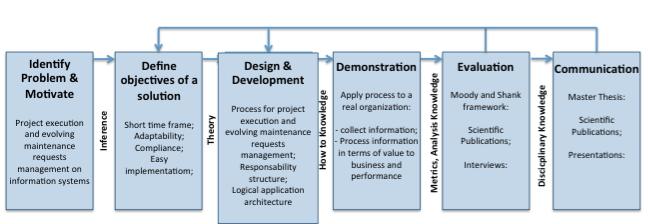
\includegraphics[width=\textwidth]{img/DSRMProcessMapping.png}
\caption{Project Mapping to DSRM Process}
\end{figure}


In figure 1 we present the mapping between the DSRM process and this project research methodology. The next sections follow the methodology steps: Section 3 (Problem contextualization) will define problem context and its importance. In section 4 and 5 we present the state of the art in frameworks and standards for management and governance processes. In section 6 we present the state of the art for market solutions on ITSM and PPM tools. In section 7 we make a solution and demonstration proposal being section 8 reserved for the evaluation methodology.\par



%!TEX root = ../report.tex

% 
% Architecture
% 

\section{Problem Contextualization}


Dealing and managing project execution and evolving maintenance requests has become one of the most important processes inside an Information Systems department, in the way it is essential a correct classification and management for the whole request life cycle until it has been fulfilled, in order to create value for the organization.\par
When a request is submitted to the information systems management, it should be classified as a project request or an evolutive maintenance. Furthermore, the organization should have defined processes to manage the whole process for request fulfillment, defining activities, expected results and responsibilities, independently of the request type.\par
The request's classification will depend on many factors. We can decide it by taking in account aspects like the risk to the business or the financial impact for the organization. In the end, it depends on aspects the organization defines as the ones which makes the distinction between a project request or evolutive maintenance.\par
After classified, we need to define the request solution in terms of processes to consider and communication channels between the project and the maintenance departments, assuming they are independent but need to be coordinated.\par
Considering the software life cycle processes, presented by the International Standard ISO/IEC 12207\cite{ISO12207} analyzed in more detail in section 5.1, we can divide this processes in two groups: Software Specific Processes and System Context processes.\par
The system context processes are more focused on systems' engineering, providing a system context for dealing with a standalone software product or service of a software system. The software specific processes are, on the other hand, used for implementing a software product or service that is an element of a larger system. \par 
The main challenge of our problem is to identify and implement the necessary processes that are important for our objectives, defining activities and responsibilities for the requests' management and its solution.\par
As long as we are dealing with an established organization in the market, we need to take in account that our processes will be implemented in an existent organizational structure. It is necessary to develop a logical application architecture, using market solutions from the area of Project Management and IT Service Support Management, that will be architecturally integrated to support our processes. We will need to assess the market solutions already available to conclude which are the best in terms of features and interest for the project. 

%!TEX root = ../report.tex

% 
% Related work
% 

\section{Related Work}

% Example citation:
In this section we will present a set of literature references on the subjects related to this thesis. We will present the most important frameworks on Information Systems Management and Governance. This process has the objective to come up with a choice of a frameworks or a set of them to implement our processes for project and maintenance management\par
In terms of logical application architectures, we will provide an analysis of the main features of a set of Project Management and Information Technologies Service Management solutions available in the market. Our objective is to conduct an comparative analysis relating all the solutions and choose the ones that best fit our purposes for use on an logical application architecture.  

\subsection{Frameworks for Information Technologies Governance and Management}

In this section we will present the three frameworks we consider the most relevant for this thesis: COBIT 5, ITIL V3 and PMBOK. This three frameworks provide, from different perspectives, guides and principles for IT Governance and Management, providing processes for achieving a successful implementation of this principles in an organization.\par


\subsubsection{IT Governance and IT Management}

One important concept to define is the difference between IT Governance and IT management. They are many times confused and some authors already tried to explain the difference between the two concepts.\par
Considering the definition given by Van Grembergen \textit{et al.}, ``''IT Management is focused on the internal effective supply of IT services and products and the management of present IT operations. IT Governance in turn is much broader, and concentrates on performing and transforming IT to meet present and future demands of the business (internal focus) and the business' customers (external focus).``''.\par
 Considering the COBIT 5 view for this question, it makes a clear distinction between governance and management, in the way these two disciplines encompass different types of activities, require different organizational structures and serve different purposes.\par
 Governance ensures that stakeholder needs, conditions and options are evaluated to determine balanced, agreed-on enterprise objectives to be achieved; setting direction through prioritisation and decision making; and monitoring performance and compliance against agreed-on direction and objectives.Management plans, builds, runs and monitors activities in alignment with the direction set by the governance body to achieve the enterprise objectives.\par

\begin{figure}
\centering
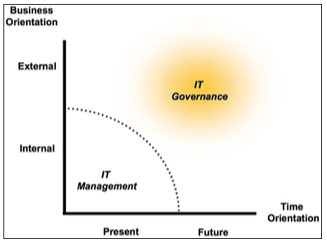
\includegraphics[width=0.6\textwidth]{img/ITGovernanceAndManagement.png}
\caption{IT Governance and IT Management}
\end{figure}


 Considering both definitions and the figure 1, we can conclude that IT Governance has a bigger dimension that IT Management, but are disciplines that need to be related and complementary to achieve success inside an organization.

\subsubsection{COBIT 5}

Control Objectives for Information and Related Technology (COBIT) is a framework created by the Information Systems Audit and Control Association (ISACA) for IT Management and IT Governance.\par
COBIT 5 provides a comprehensive framework that assists enterprises in achieving their objectives for the governance and management of enterprise IT. Simply stated, it helps enterprises create optimal value from IT by maintaining a balance between realizing benefits and optimizing risk levels and resource use \cite{2012cobit}. 
The framework is built on five basic principles:

\begin{itemize}
  \item Meeting the Stakeholders Needs 
  \item Covering the Enterprise End-to-end
  \item Applying a Single, Integrated Framework
  \item Enabling a Holistic Approach
  \item Separating Governance from Management
\end{itemize}


It also defines seven enablers, explained by COBIT as factors that, individually and collectively, influence whether governance and management over enterprise will work or not. This enablers can be categorized as:

\begin{itemize}
  \item Principles, Policies and frameworks 
  \item Processes 
  \item Organizational structures
  \item Culture, ethics and behavior 
  \item Information
  \item Services, infrastructure and applications
  \item People, skills and competencies
\end{itemize}

\begin{figure}
\centering
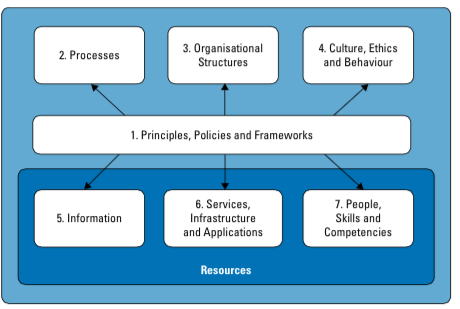
\includegraphics[width=0.7\textwidth]{img/Enablers.png}
\caption{COBIT 5 enablers}
\end{figure}

Image 2 presents the COBIT 5 enablers previous defined and how they relate among themselves int terms of its importance for organization. Each enabler has stakeholders, a set of goals, a life cycle and for each can be defined good practices.\par

\begin{figure}
\centering
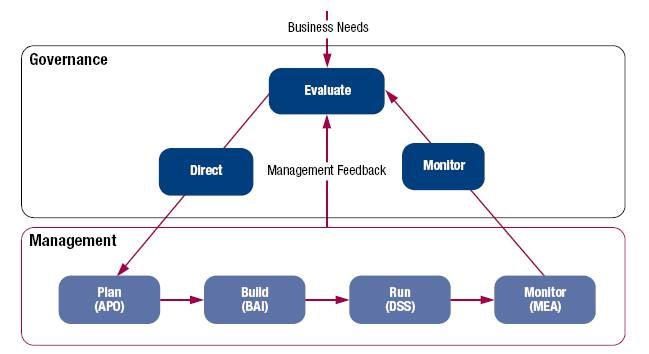
\includegraphics[width=0.9\textwidth]{img/COBITProcesses.jpg}
\caption{COBIT 5 domains}
\end{figure}

Considering figure 3, COBIT 5 process reference model considers two big domains of processes: Governance and Management. The governance domain contains five processes in the domain evaluate, direct and monitor(EDM). The management domain has four internal domains of processes:Align, Plan and Organise(APO), Build, Acquire and Implement(BAI), Deliver, Service and Support (DSS) and Monitor, Evaluate and Assess(MEA).\par
All processes for management and governance are presented in the appendix and all the implementation details explained in COBIT 5: Enabling Processes, A detailed reference guide to the processes defined in the COBIT 5 process reference model. This includes the COBIT 5 goals cascade, a process model explanation, governance and management practices, and the process reference model\cite{2012cobitEP}.\par
COBIT 5 includes a process capability model based on ISO/IEC 15504 Software Engineering - Process Assessment standard. [REFERENCE HERE] This models allow to measure the current level of maturity of enterprise processes, presenting the gap between the current level and the desired one the enterprise wants to achieve. This new capability model is an improvement of the previous on COBIT 4.1, being more simplified and compliant with a generally accepted process assessment standard.\par
Relating to other frameworks and standards, COBIT tries to establish a framework that is compliant with the most widely accepted standards in IT Governance and Management. In figure 4 we can see the standards COBIT 5 relates by processes domain, with special attention to ITIL V3, ISO/IEC 20000, PMBOK and CMMI, that are closely related to this thesis problem. This compliance with other standards is fundamental for a widely adoption of COBIT 5, in the way it tries to establish goals, metrics, practices, roles, inputs and outputs for each process, making it necessary being compliant with international standards. This is will improve COBIT application and acceptance.\par

\subsubsection{COBIT 5 critical analysis}

The COBIT 5 is one of the most interesting frameworks widely accepted by organizations in the IT management and Governance Area. It arises as the main framework for establishing processes to guide us on management and governance and establish ways to control them. However, its a complex framework that needs time and practice to be fully implemented.\par
For this thesis project, we will consider only the domains relevant for our objectives, making a selection of the processes we pretend to implement. This will allow us to get the bigger value COBIT has to offer, making it possible, in the time-frame available, achieve our implementation objectives.\par
One important aspect of the use of COBIT is that it provides a more business and strategic view of IT on organizations, presenting a lack of operational approach to some themes that are relevant for our project. To overcome this, we will analyze a more operational framework on IT service management, the ITIL V3 framework and a project management guide considered by the main specialists on the area as the reference for project management, the Project Management Book of Knowledge.\par

\begin{figure}
\centering
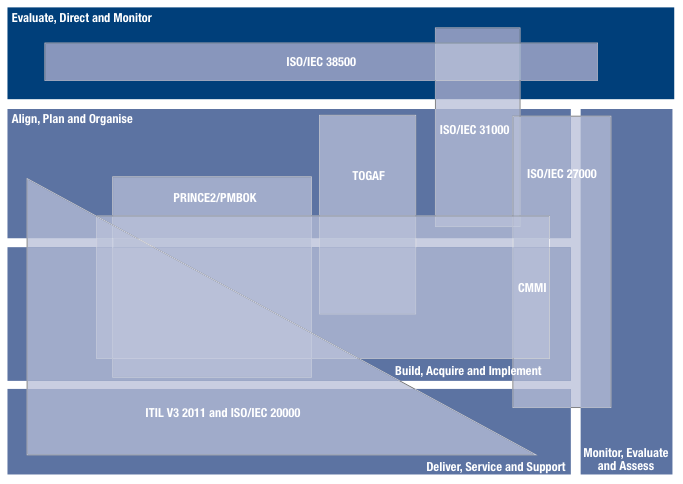
\includegraphics[width=0.9\textwidth]{img/COBITOtherFrameworks.png}
\caption{COBIT 5 coverage on other frameworks}
\end{figure}

\subsubsection{ITIL V3}

First developed in the 1980s by the Office of Government Commerce (OGC), a branch of the British Government, ITIL defines processes at a high level. It is left to the organizations to implement the processes in the manner most suitable to their particular situations and needs.\par
ITIL is becoming a de facto standard worldwide as organizations adopt it as their guideline for establishing IT service management (ITSM) processes. IT organizations can use the guidance provided by ITIL to transform their service management capabilities into strategic assets, those that provide the basis for core competence, distinctive performance, durable advantage, and qualifications to participate in business opportunities.\par
The ITIL service management practices are comprised of three main sets of products and services: ITIL service management practices (core guidance), ITIL service management practices (guidance specific to industry sectors, organization types, operating models and technology architectures) and ITIL web support services.\par

\begin{figure}
\centering
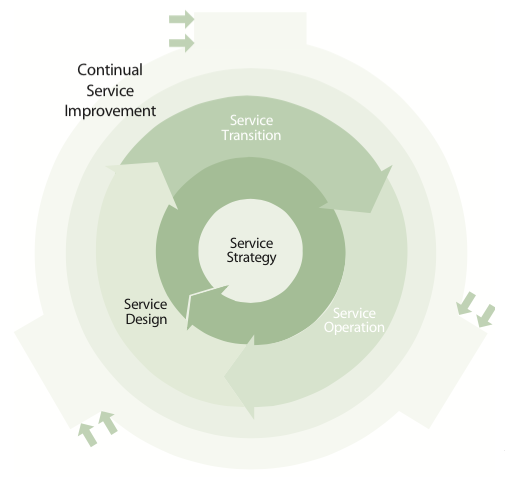
\includegraphics[width=0.7\textwidth]{img/ITILVolumes.png}
\caption{COBIT 5 coverage on other frameworks}
\end{figure}

The core set, presented in figure XXX and the one we will consider for this thesis, consists of six publications: Introduction to ITIL Service Management Practices, Service Strategy, Service Design, Service Transition, Service Operation and Continual Service Improvement. Each one of this volumes is composed by practice fundamentals and principles, Lifecycle processes and activities, Supporting organization structures and roles, Technology considerations, Practice implementation and Challenges, risks and critical success factors.

\paragraph{\textbf{Service Strategy}} provides guidance on how to view service management not only as an organizational capability but as a strategic asset. Guidance is provided on the principles underpinning the practice of service management which are useful for developing service management policies, guidelines and processes across the ITIL Service Lifecycle. The processes included in Service Strategy volume are:

\begin{itemize}
  \item Financial Management
  \item Service Portfolio Management 
  \item Demand Management
\end{itemize}

\paragraph{\textbf{Service Design}} provides guidance for the design and development of services and service management practices. It covers design principles and methods for converting strategic objectives into portfolios of services and service assets. The scope of Service Design is not limited to new services. It includes the changes and improvements necessary to increase or maintain value to customers over the lifecycle of services, the continuity of services, achievement of service levels, and conformance to standards and regulations. The processes included in Service Design volume are:

\begin{itemize}
  \item Service Catalogue Management
  \item Service Level Management 
  \item Capacity Management
  \item Availability Management
  \item IT service Continuity Management
  \item Information Security Management 
  \item Supplier Management
  \item Application Management
  \item Data and Information Management
  \item Business Service Management
\end{itemize} 

\paragraph{\textbf{Service Transition}} provides guidance for the development and improvement of capabilities for transitioning new and changed services into live service operation. This publication provides guidance on how the requirements of Service Strategy encoded in Service Design are effectively realized in Service Operation while controlling the risks of failure and disruption.The processes included in Service Transition volume are:

\begin{itemize}
  \item Change Management
  \item Service asset and Configuration Management
  \item Release and deployment Management
  \item Knowledge Management
  \item Stakeholder Management
  \item Transition Planning 
  \item Support and Service Evaluation 
\end{itemize} 

\paragraph{\textbf{Service Operation}} embodies practices in the management of the day-to-day operation of services. It includes guidance on achieving effectiveness and efficiency in the delivery and support of services to ensure value for the customer and the service provider. Strategic objectives are ultimately realized through Service Operation, therefore making it a critical capability. Guidance is provided on how to maintain stability in service operations, allowing for changes in design, scale, scope and service levels.The processes included in Service Operation volume are:

\begin{itemize}
  \item Event Management
  \item Incident Management
  \item Request Management
  \item Problem Management
  \item Access management
\end{itemize} 

\paragraph{\textbf{Continual Service Improvement}} provides instrumental guidance in creating and maintaining value for customers through better design, transition and operation of services. It combines principles, practices and methods from quality management, change management and capability improvement. Organizations learn to realize incremental and large-scale improvements in service quality, operational efficiency and business continuity. Guidance is provided for linking improvement efforts and outcomes with service strategy, design and transition. The processes included in Service Operation volume are:

\begin{itemize}
  \item The 7-Step Improving Process
  \item Service Level Management
\end{itemize} 

\par Not different from COBIT,  ITIL takes public frameworks and standards as a form of the organization to have advantage on the market. Organizations should build their proprietary knowledge on top of a body of knowledge based on public frameworks and standards. Collaboration and coordination across organizations are easier because of shared practices and standards. According to research by the UK Department of Trade and Industry (DTI), the value to the UK economy from standards is estimated to be about \textsterling2.5 billion per annum \cite{McNeillis01112005}.\par
For related standards and frameworks to ITIL V3, we have ISO/IEC 20000 (service management system standards), ISO/IEC 27001 (standard providing requirements for an information security management system), PMBOK (manual for a set of standard terminology and guidelines for project management) and COBIT, already presented. This are the standards we will cover for out thesis by being directly related to ITIL V3 and its implementation.


\subsubsection{ITIL V3 critical analysis}

One crucial aspect for the importance of ITIL on this thesis is the operational view that it provides for IT Service Management. ITIL tries to focus on more management details, providing a more practical guidance for implementation. It is focused on IT Service Management and presents concrete guidance for managing services during its lifecycle. De Haes and Van Grembergen state that COBIT tells what to do and ITIL explains how to do it, what makes COBIT adopting a process-focused approach and ITIL a service level-oriented one \cite{ITGovAndMech}.\par
The main objective to include ITIL knowledge for this thesis is to provide a complementary guidance on IT management, enhancing the business oriented view of COBIT with a operational view. COBIT 5 will allow us to take advantage of this complementarity, related to the concern of ISACA to make it more compliant with other frameworks, including COBIT, on the new version (relating to COBIT 4.1). 

\subsubsection{PMBOK: A Guide to the Project Management Book of Knowledge}









%!TEX root = ../report.tex

% 
% Architecture
% 

\section{Solution's Architecture Proposal}

Considering this project's problem and the objectives presented in problem contextualization section, we want to develop a process architecture for project and maintenance management to be applied to an Information Systems administration, supported by a logical application architecture.\par
As long as this project is aligned with a real-case scenario for an organization, we will take the main design decisions considering the stakeholders' needs and concerns for this project, namely the processes to consider for the architecture development and the solutions chosen for integrating the logical application architecture. It will also provide a demonstration scenario for our solution, allowing us to achieve the demonstration and evaluation steps of the DSRM process.\par 



\subsection{Real-case Scenario}

The real-case organization scenario will provide constraints and assumptions for this project, made available by the organization's stakeholders. Being so, some design decisions were made considering specific requirements from this scenario.\par
We are dealing with an organization from the utilities sector of Business (Energy), composed by a unique administration for Applications (software) area. This administration will receive two types of requests: project execution and evolving maintenance requests.\par
Considering the stakeholders for this project, we have two types: Internal and External. Considering internal stakeholders, we have the Business area, composed by the organization administration (Sponsor of this project), the financial and logistic departments, and the Technology area, composed by the Information Systems department (Project execution and Maintenance departments). Considering the external stakeholders, we have the third-parties responsible for project implementation, suppliers, consumers and regulatory entities.\par
Project Execution department will outsource project implementation to a third-party but internally will maintain processes for project management, independent from the third-party. Evolving maintenance requests are filtered by a Help-Desk service, Wherefore only the major changes requests arrive to the evolving maintenance department.\par
A project only enters in production phase after approval from the maintenance department. When in production phase, project belongs to the maintenance department. It can, accordingly with a strategical plan previously defined, outsource the maintenance's implementation, being only responsible for its management.\par
This real-case scenario will allow us to extract some requirements and also take design decisions accordingly to organization's stakeholders' needs and concerns, deciding which processes must be included in the processes architecture and the ones we should not focus, to reduce unnecessary complexity.\par


\subsection{Process Architecture}

Taking as reference ISO/IEC 12207, detailed in section 5.1, that standardizes the processes for the whole life cycle of software, we will present the areas we will address in our processes architecture and the reasons for not considering others.\par
The two main processes areas we can address are governance and management processes. Considering the extensibility of both, we could not focus on the two, giving the time-frame available. Being so, we decided, accordingly with the stakeholders, to not detail governance processes. This type of processes need maturation and organization's insight, being too much complex in the scope of this project. Areas as organization strategy or project portfolio will not be addressed.\par 
Despite this, there are governance processes that will have direct influence on the subjects covered by this project, namely risk, budget and quality management. These subjects will be addressed considering a more operational approach, assuming that organization's strategy for this areas is already defined, being our mission design processes that implement it in practice.\par
We are considering the use of BPMN 2.0 (Business Process Model and Notation) for processes modeling. It provides a graphical representation for specifying business processes, being the standard for business processes modeling. Due to its large adoption by organizations for business processes' specification, it is the best option for designing a processes architecture. \par


\subsubsection{Processes definition}

Using an interview approach with the organization's stakeholders for a more deeper analysis on the problem scope, we defined the areas of interest we need to cover. This areas can change during project execution phases, since requirements are volatile and can be changed. Also, more areas can be covered in the future, if we consider it brings an added value for this architecture.\par
In Figure 18 we can observe the processes of interest for this project highlighted from the ISO/IEC 12207 international standard. As explained before, processes directly related to governance areas are not considered for this project due to its increased complexity. As consequence, Agreement processes and Organizational Project-Enabling processes are outside the scope for this project.\par
Technical Processes and Software Implementation processes are also not considered in the scope, based on the requirements presented by the stakeholders and the organization scenario provided. As stated in section 7.1, we will assume these processes will be either outsourced, or managed by the organization according to already defined processes for that purpose.\par
Software Reuse Processes are also outside the scope of this project. It is a shared opinion of stakeholders that this processes are not related to this project's problem and would only increase its complexity without adding any value.\par
The processes we will address in detail are the Project processes and the Software Support processes, directly related to project and maintenance management. It constitutes the core of this project and is fundamental for establishing the proposed processes architecture.\par
Regarding Project processes, and accordingly to the concerns extracted from the stakeholders' interview, we will consider all processes with exception of configuration management process and measurement process, that are not in the scope of interest for this particular project. Considering Software Support Processes, we will only address the Software Configuration Management process and the Software Validation process.\par


\begin{figure}[h!]
\centering
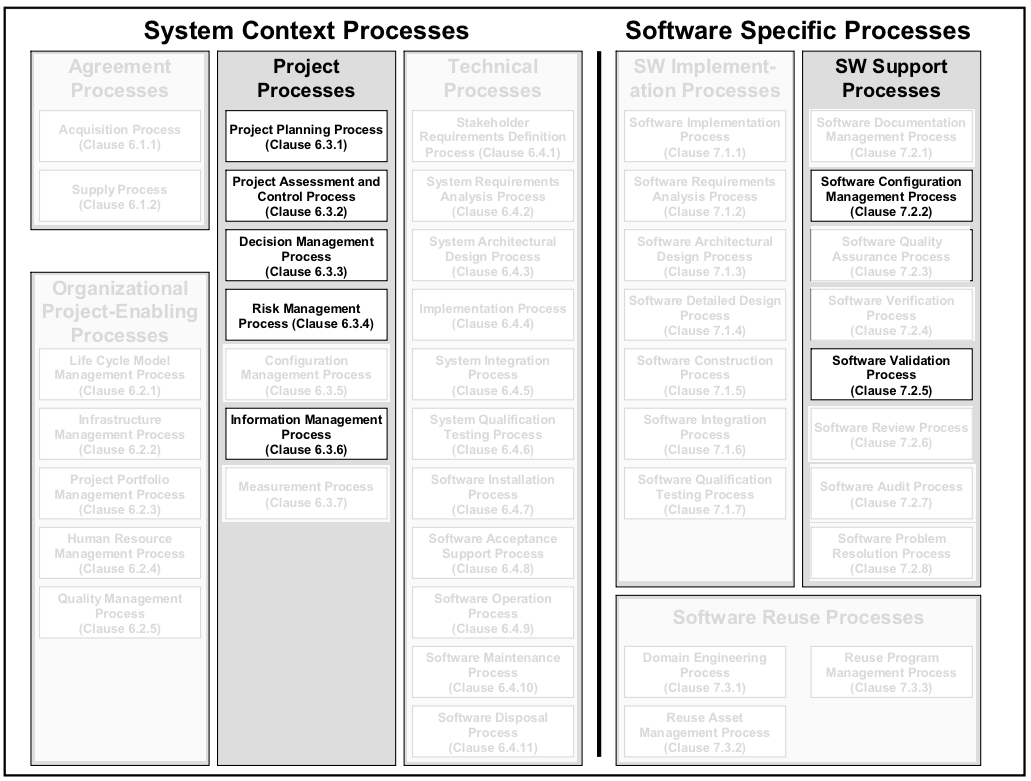
\includegraphics[width=0.8\textwidth]{img/ISO12207ProcessesImplemented.png}
\caption{Processes areas considered for this project. Adapted from \cite{ISO12207}.}
\end{figure}

Apart from processes presented by ISO/IEC 12207, the stakeholders presented specific concerns regarding processes on Capacity Management, Issues Management, Financial Management and Document Management. They need to be taking in account on this project's scope considering stakeholders' needs.\par
Capacity Management, as stated in \cite{itilSD}, ``ensure that cost-justifiable IT capacity in all areas of IT always exists and is matched to the current and future agreed needs of the business, in a timely manner.''. Deals with performance achievement and capacity availability, considering resources and services itself. It tries to balance costs against resources needed and supply against demand.\par
The main areas are Business Capacity Management (requirements for service and IT infrastructure), Service Capacity Management (performance and capacity management of IT services operation) and Component Capacity Management (performance, capacity and utilization management of individual IT technology components).\par
Issues Management is the process of identifying and resolving issues, as staff, suppliers, technical or material problems. Many times confused with risks, they can arise from project processes with no warning or no expectation at all. Most organizations find difficult to manage issues from an effectively manner and many times it a process that is not implemented across the complete organization, making more difficult its resolution.\par
Financial Management, as stated in \cite{itilSS}, ``provides the business and IT with the quantification, in financial terms, of the value of IT Services, the value of the assets underlying the provisioning of those services, and the qualification of operational forecasting''. Core areas for IT Financial Management are Budgeting (Expenditures planning and controlling), IT accounting (Cost analysis on IT services providing) and Charging (Costs assignment to IT services provided). Financial Management is a complex area and we need a more deeper analysis on its importance for our architecture, in order to remove unnecessary complexity.\par
Documentation Management corresponds to an area that deals with all documentation concerns on an organization, from technical to project management documentation. This area groups processes for plan, production, tracking and communication of documents produced by the organization in project and maintenance contexts. This processes are also related to the supporting artifacts we want to develop.\par
In Table 2 we present the processes we will consider for this project and a description of some activities each process implements.

\begin{table}[h!]
\centering
\resizebox{0.9\textwidth}{!}{%
\begin{tabular}{|c|l|}
\hline
\textbf{Processes} & \multicolumn{1}{c|}{\textbf{Description}} \\ \hline
\textbf{Project Planning} & \begin{tabular}[c]{@{}l@{}}Scope and goals definition;\\ Requirements establishment;\\ Activities and deliverables identification;\\ Schedule definition;\\ Resources identification;\\ Responsibilities assignment;\\ Quality, Risk and Cost Analysis;\end{tabular} \\ \hline
\textbf{Project Assessment and Control} & \begin{tabular}[c]{@{}l@{}}Project monitoring;\\ Project control;\\ Project assessment;\end{tabular} \\ \hline
\textbf{Decision Management} & \begin{tabular}[c]{@{}l@{}}Decision Planning;\\ Decision analysis;\\ Decision tracking;\end{tabular} \\ \hline
\textbf{Risk Management} & \begin{tabular}[c]{@{}l@{}}Risk Management planning;\\ Risk Profile Management;\\ Risk Analysis;\\ Risk Treatment;\\ Risk Monitoring;\\ Risk Management process evaluation;\end{tabular} \\ \hline
\textbf{Capacity Management} & \begin{tabular}[c]{@{}l@{}}Capacity Plan definition;\\ Performance Monitoring;\\ Performance Analysis;\\ Performance tuning;\end{tabular} \\ \hline
\textbf{Issues Management} & \begin{tabular}[c]{@{}l@{}}Issue Identification;\\ Issue Prioritization;\\ Issue Resolution;\\ Issue Communication;\end{tabular} \\ \hline
\textbf{Financial Management} & \begin{tabular}[c]{@{}l@{}}Budgeting definition;\\ IT Accounting planning;\\ Charging planning;\\ Financial control;\\ Financial communication;\end{tabular} \\ \hline
\textbf{Documentation Management} & \begin{tabular}[c]{@{}l@{}}Documentation definition;\\ Documentation production;\\ Documentation validation;\\ Documentation communication;\\ Documentation tracking;\end{tabular} \\ \hline
\textbf{Software Configuration Management} & \begin{tabular}[c]{@{}l@{}}Software configuration management plan developing;\\ Configuration Identification;\\ Configuration Control;\\ Configuration Status Accounting;\\ Configuration Evaluation;\end{tabular} \\ \hline
\textbf{Software Validation} & \begin{tabular}[c]{@{}l@{}}Validation plan definition;\\ Test requirements, test cases and test specifications preparation;\\ Tests Execution;\\ Software validation against the requirements execution;\end{tabular} \\ \hline
\end{tabular}
}
\vspace{2mm}
\caption{Processes areas and main activities.}
\label{my-label}
\end{table}



\subsubsection{Processes Mapping to frameworks}

In this section we will present how each one of the processes in the scope for this project is addressed and mapped into the frameworks and standards presented in section 4 and 5. This will provide us an initial guidance on how we should approach the problem, analyzing what objectives are already covered by the frameworks and which ones need more original work.\par
Our objective is to use only the important knowledge from sections 4 and 5 for this project, reducing the complexity of implementing a complete framework for the organization. In Table 3 we present the mapping between each processes group in the scope for this project with the framework or standard that covers some aspects for it:\par

\begin{table}[h!]
\centering
\resizebox{\textwidth}{!}{%
\begin{tabular}{|l|c|c|c|c|c|c|c|c|c|c|c|c|c|}
\hline
\multicolumn{1}{|c|}{} & \multicolumn{4}{c|}{\textbf{COBIT 5 Domains}} & \multicolumn{5}{c|}{\textbf{ITIL V3 Volumes}} &  &  &  &  \\ \cline{2-10}
\multicolumn{1}{|c|}{\multirow{-2}{*}{\textbf{Processes}}} & \textbf{APO} & \textbf{BAI} & \textbf{DSS} & \textbf{MEA} & \textbf{SS} & \textbf{SD} & \textbf{SO} & \textbf{ST} & \textbf{CSI} & \multirow{-2}{*}{\textbf{PMBOK}} & \multirow{-2}{*}{\textbf{\begin{tabular}[c]{@{}c@{}}ISO/IEC\\ 20000\end{tabular}}} & \multirow{-2}{*}{\textbf{\begin{tabular}[c]{@{}c@{}}ISO/IEC \\ 27000\end{tabular}}} & \multirow{-2}{*}{\textbf{\begin{tabular}[c]{@{}c@{}}ISO\\ 31000\end{tabular}}} \\ \hline
\textbf{Project Planning} & \cellcolor[HTML]{5A9D58}\checkmark & \cellcolor[HTML]{5A9D58}\checkmark &  &  &  &  &  &  &  & \cellcolor[HTML]{FD6864}\checkmark & \cellcolor[HTML]{329A9D}\checkmark &  &  \\ \hline
\textbf{Project Assessment and Control} & \cellcolor[HTML]{5A9D58}{\color[HTML]{000000} \checkmark} & \cellcolor[HTML]{5A9D58}{\color[HTML]{000000} \checkmark} & \cellcolor[HTML]{5A9D58}{\color[HTML]{000000} \checkmark} & \cellcolor[HTML]{5A9D58}{\color[HTML]{000000} \checkmark} &  &  &  &  &  & \cellcolor[HTML]{FD6864}\checkmark & \cellcolor[HTML]{329A9D}\checkmark &  &  \\ \hline
\textbf{Decision Management} & \cellcolor[HTML]{5A9D58}{\color[HTML]{000000} \checkmark} & \cellcolor[HTML]{5A9D58}{\color[HTML]{000000} \checkmark} & \cellcolor[HTML]{5A9D58}{\color[HTML]{000000} \checkmark} & \cellcolor[HTML]{5A9D58}{\color[HTML]{000000} \checkmark} & \cellcolor[HTML]{FFCC67}\checkmark &  &  &  &  & \cellcolor[HTML]{FD6864}\checkmark & \cellcolor[HTML]{329A9D}\checkmark &  &  \\ \hline
\textbf{Risk Management} & \cellcolor[HTML]{5A9D58}\checkmark &  &  &  &  & \cellcolor[HTML]{FFCC67}\checkmark &  &  &  & \cellcolor[HTML]{FD6864}\checkmark &  & \cellcolor[HTML]{329A9D}\checkmark & \cellcolor[HTML]{329A9D}\checkmark \\ \hline
\textbf{Capacity Management} & \cellcolor[HTML]{5A9D58}\checkmark & \cellcolor[HTML]{5A9D58}\checkmark &  &  &  & \cellcolor[HTML]{FFCC67}\checkmark &  &  &  &  &  &  &  \\ \hline
\textbf{Issues Management} &  &  & \cellcolor[HTML]{5A9D58}\checkmark &  &  &  & \cellcolor[HTML]{FFCC67}\checkmark &  &  &  &  &  &  \\ \hline
\textbf{Financial Management} & \cellcolor[HTML]{5A9D58}\checkmark &  &  &  & \cellcolor[HTML]{FFCC67}\checkmark &  &  &  &  &  &  &  &  \\ \hline
\textbf{Documentation Management} & \cellcolor[HTML]{5A9D58}\checkmark & \cellcolor[HTML]{5A9D58}\checkmark &  &  &  &  &  &  &  & \cellcolor[HTML]{FD6864}\checkmark &  & \cellcolor[HTML]{329A9D}\checkmark &  \\ \hline
\textbf{Software Configuration Management} &  & \cellcolor[HTML]{5A9D58}\checkmark &  &  &  &  &  & \cellcolor[HTML]{FFCC67}\checkmark &  &  &  &  &  \\ \hline
\textbf{Software Validation} & \cellcolor[HTML]{5A9D58}\checkmark &  &  &  &  &  &  & \cellcolor[HTML]{FFCC67}\checkmark &  & \cellcolor[HTML]{FD6864}\checkmark &  &  &  \\ \hline
\end{tabular}
}
\vspace{2mm}
\caption{Processes Mapping to frameworks and standards.}
\label{my-label}
\end{table}


\subsubsection{Processes Supporting artifacts}

Considering the processes architecture we want to develop, we need some artifacts to support this processes, namely communication and decisions artifacts that will allow us to support the activities' inputs and outputs. For this, we will identify all artifacts needed, clearly defining its purpose, content and participants.\par
This artifacts will be defined during the designing of the process architecture. The frameworks and standards previously presented define some of them, being our work to address new artifacts that are not already covered and adapt others to better suit to our objectives.\par

\subsubsection{Responsibility Structure}

The developed architecture needs to have an inherent responsibility structure, defining the processes' participants accounted for decisions and activities. This structure is particularly important when considering we are dealing with a real-case organization, having an organizational structure already defined and for which our processes should be applied.\par
For designing this responsibility structure we will consider the work already done in responsibility assignment for the frameworks and standards previously presented. Despite that, we need also to have some original work on this area, considering we are not implementing directly any of those frameworks. This work will be accomplished during the processes' design and taking in account the common responsibility structures on IT organizations.\par 

\subsection{Logical Application Architecture}

A proposal for a logical application architecture is one of the objectives of this project, being important to support the processes architecture. To achieve this, we evaluated a set of PPM and ITSM solutions available in the market with the objective of achieving a proposal of applications that can be a part of this architecture.\par
We will only consider proprietary solutions, due to explicit requirements from the organization's stakeholders. This was a precondition that we did not take in account in the state of the art on section 6 but that in this phase will restrict our PPM and ITSM solutions' proposal.\par 
For evaluation purposes, we used Gartner and Forrester research, presented in section 6, that allow us to independently evaluate how these tools stand a position in the PPM and ITSM Market and also what are the solutions more complete in terms of features and capabilities.\par
In this section we will present the solutions we consider the best for our objectives, being part of a proposal for the project's stakeholders. After deciding what solution we will consider for this project, we need to design a logical application architecture, describing how processes are supported and integrated.\par

\subsubsection{PPM Tools}

For PPM solutions, that we evaluate in section 6.2, we used the Gartner Magic Quadrant and the Forrester Wave methodologies for evaluation.\par
In Magic Quadrant results, that performs an evaluation of the PPM solutions' providers adequacy to the market, we will just consider the leaders quadrant, composed by Planview, Compuware, CA, HP, Oracle and Microsoft. Planview and CA are the suppliers with the best results but are closely followed by the rest. A deeper analysis on strengths and cautions presented by Gartner for each one of this solutions is presented in \cite{magicQuadrantPPM}.\par
For the Forrester Wave results, that evaluates providers by criteria and respective weightings, we will consider the two models explained in section 6.2.2, the above-the-line and below-the-line. For the first one, the leaders quadrant is composed by Planview, CA Technologies, HP and Daptiv. All presents good results but is CA Technologies who is the most complete provider, in terms of current offering, strategy and market presence. Other providers present better results in some of this criteria but are substantially worse in others. For the below-the-line evaluation, we have CA Technologies and Planview very close to each other and HP with an excellent result in strategy criteria. Microsoft, Rally and Daptiv are also part of the leaders, but with results slightly worse.\par
In Table 3 we can observe the PPM Tools Evaluation results. In green we have the solutions we consider the best for this project taking in account the evaluation results. We also present the alternatives in orange. CA Technologies with CA Clarity PPM, Planview with Planview Enterprise and HP with HP PPM Center are the solutions we will purpose for the PPM Tool to consider for this project.


\begin{table}[h!]
\centering
\resizebox{\textwidth}{!}{%
\begin{tabular}{|c|c|l|c|c|l|}
\hline
 & \multicolumn{2}{c|}{} & \multicolumn{3}{c|}{\textbf{Forrester Wave}} \\ \cline{4-6} 
\multirow{-2}{*}{\textbf{Solutions Providers}} & \multicolumn{2}{c|}{\multirow{-2}{*}{\textbf{\begin{tabular}[c]{@{}c@{}}Gartner Magic\\ Quadrant\end{tabular}}}} & \multicolumn{1}{l|}{\textbf{Above-The-Line}} & \multicolumn{2}{l|}{\textbf{Below-The-Line}} \\ \hline
\rowcolor[HTML]{5A9D58} 
\textbf{CA Technologies} & \multicolumn{2}{c|}{\cellcolor[HTML]{5A9D58}Leader} & Leader & \multicolumn{2}{c|}{\cellcolor[HTML]{5A9D58}Leader} \\ \hline
\rowcolor[HTML]{5A9D58} 
\textbf{Planview} & \multicolumn{2}{c|}{\cellcolor[HTML]{5A9D58}Leader} & Leader & \multicolumn{2}{c|}{\cellcolor[HTML]{5A9D58}Leader} \\ \hline
\rowcolor[HTML]{5A9D58} 
\textbf{HP} & \multicolumn{2}{c|}{\cellcolor[HTML]{5A9D58}Leader} & Leader & \multicolumn{2}{c|}{\cellcolor[HTML]{5A9D58}Leader} \\ \hline
\rowcolor[HTML]{FFCB2F} 
\textbf{Microsoft} & \multicolumn{2}{c|}{\cellcolor[HTML]{FFCB2F}Leader} & Strong Performer & \multicolumn{2}{c|}{\cellcolor[HTML]{FFCB2F}Leader} \\ \hline
\textbf{Oracle} & \multicolumn{2}{c|}{Leader} & - & \multicolumn{2}{c|}{-} \\ \hline
\textbf{Compuware} & \multicolumn{2}{c|}{Leader} & - & \multicolumn{2}{c|}{-} \\ \hline
\textbf{Rally} & \multicolumn{2}{c|}{-} & Strong Performer & \multicolumn{2}{c|}{Leader} \\ \hline
\textbf{Daptiv} & \multicolumn{2}{c|}{-} & Leader & \multicolumn{2}{c|}{Leader} \\ \hline
\end{tabular}
}
\vspace{2mm}
\caption{PPM Tools evaluation results.}
\label{my-label}
\end{table}

\vspace{10mm}

\subsubsection{ITSM Tools}

For ITSM solutions, that we evaluated in section 6.3, we used the Magic Quadrant , the Critical Capabilities and the Forrester Wave methodologies for evaluation.\par
In Magic Quadrant results we will just consider the leaders and challengers quadrants, composed by ServiceNow and BMC Software for the leaders and Cherwell and CA Technologies for challengers. ServiceNow is the best provider in terms of ability to execute with some advantage to concurrency but really close of BMC Software in terms of completeness of vision. Cherwell Software and CA Technologies present a considering lower result for completeness of vision considering the leaders quadrant. A deeper analysis on strengths and cautions presented by Gartner for each one of this solutions is presented in \cite{magicQuadrantITSM}.\par
In Critical Capabilities results, we will only consider the High-Maturity, Digital Workplace and Total ITSM Use Cases, the ones that are more adequate to our objectives and to the organization's scenario. We will also only consider the solutions provided by the suppliers in the leaders and challengers quadrants presented by Gartner. In all the use cases considered, BMC Remedy ITSM Suite and ServiceNow IT Service Automation suite have the higher scores, being followed by some distance by CA Service Management and Cherwell Software Service Management.\par
For the Forrester Wave results, we have Cherwell Software and Service Now as the leaders, very close to each other and with a very good result in terms of market presence. BMC Software and CA Technologies are considered Strong Performers, but at some distance of the other two. Forrester establishes big differences between the two leaders providers and the two strong contenders in terms of the three criteria considered.\par
In Table 4 we can observe the ITSM Tools Evaluation results. In green we have the solution we consider the best for this project taking in account the evaluation results. ServiceNow with ServiceNow IT Service Automation is the solution we will purpose for the ITSM Tool to consider for this project. We also present other alternatives in orange. It should be taken special attention to CA Technologies tool as alternative solution if we consider the CA Technologies PPM tool due to easier integration between the PPM and ITSM tools.\par


\begin{table}[h!]
\centering
\resizebox{\textwidth}{!}{%
\begin{tabular}{|c|c|c|c|c|c|}
\hline
 &  & \multicolumn{3}{c|}{\textbf{Gartner Critical Capabilities}} &  \\ \cline{3-5}
\multirow{-2}{*}{\textbf{\begin{tabular}[c]{@{}c@{}}Solutions\\ Providers\end{tabular}}} & \multirow{-2}{*}{\textbf{\begin{tabular}[c]{@{}c@{}}Gartner\\ Magic \\ Quadrant\end{tabular}}} & \textbf{\begin{tabular}[c]{@{}c@{}}High\\ Maturity\\ UC\end{tabular}} & \textbf{\begin{tabular}[c]{@{}c@{}}Digital \\ Workplace \\ UC\end{tabular}} & \textbf{\begin{tabular}[c]{@{}c@{}}Total\\  ITSM\\ Use Case\end{tabular}} & \multirow{-2}{*}{\textbf{\begin{tabular}[c]{@{}c@{}}Forrester \\ Wave\end{tabular}}} \\ \hline
\rowcolor[HTML]{5A9D58} 
\textbf{ServiceNow} & Leaders & 3,68 & 3,49 & 3,56 & Leader \\ \hline
\rowcolor[HTML]{FFCC67} 
\textbf{Cherwell Software} & Challengers & 3,15 & 3,12 & 3,22 & Leader \\ \hline
\rowcolor[HTML]{FFCC67} 
\textbf{BMC Software} & Leaders & 3,74 & 3,49 & 3,52 & Strong Performers \\ \hline
\rowcolor[HTML]{FFCC67} 
\textbf{CA Technologies} & Challengers & 3,39 & 3,31 & 3,22 & Strong Performers \\ \hline
\end{tabular}
}
\vspace{2mm}
\caption{ITSM Tools evaluation results.}
\label{my-label}
\end{table}


%!TEX root = ../report.tex

% 
% Evaluation
% 

\section{Work's Evaluation Methodology}

This section corresponds to the ``Evaluation'' phase of DSRM methodology. We will present how we intent to evaluate our solution. For this project, besides the demonstration evaluation, where we will apply our processes to a real case scenario of an information systems administration of an organization, we will evaluate our solution using the Moody and Shanks Framework \cite{moody2003improving}, a framework to evaluate the quality of data models.\par
We also pretend to evaluate our processes through interviews with the main organization's scenario stakeholders of this project, considering their opinion on the processes' suitability to the problem purposed. This will allow us to have feedback from the demonstration and evaluation steps of the DSRM process.\par
Finally, and considering also the communication step of DSRM process, we will submit articles to conferences and journals where our solution will be evaluated and where we can receive feedback from specialists in the area. This articles will be developed in conformance with the conferences' and journals' calendar, being necessary to analyze the available options considering our project's calendar.\par

\subsection{Moody and Shanks Framework}

This framework presents a set of metrics to evaluate and improve quality of data models. It has arise from the necessity of guidelines to evaluate quality of data models, trying to achieve agreement between experts on what is a good quality model. This framework consists of five primary constructs:

\begin{itemize}
\item \textbf{Quality factors} are the characteristics that contribute to the overall quality of the data model.
\item \textbf{Stakeholders} are people involved in developing or using the data model, and therefore have an interest in its quality.
\item \textbf{Quality metrics} define ways of measuring particular quality factors.
\item \textbf{Weightings} define the relative importance of different quality factors and are used to make trade-offs between them.
\item \textbf{Improvement strategies} are techniques for improving the quality of data models with respect to one or more quality factors.
\end{itemize}

For quality factors, that define how can we measure the quality of our model, this framework presents:

\begin{itemize}
\item \textbf{Completeness} refers to whether the data model contains all user requirements.
\item \textbf{Simplicity} means that the data model contains the minimum possible entities and relationships.
\item \textbf{Flexibility} is defined as the ease with which the data model can cope with business and/or regulatory change.
\item \textbf{Integration} is defined as the consistency of the data model with the rest of the organization's data.
\item \textbf{Understandability} is defined as the ease with which the concepts and structures in the data model can be understood.
\item \textbf{Implementability} is defined as the ease with which the data model can be implemented within the time, budget and technology constraints of the project.
\end{itemize}

For each quality factor, a set of metrics are presented for evaluation in \cite{moody1998metrics}. The objective of this metrics is to refine these quality factors in specific and concrete measures for evaluating the quality of data models.\par
Our objective is to use this framework on our final solution, analyzing the metrics presented in \cite{moody1998metrics} to evaluate each quality factor and how it is achieved in our solution, providing a well-defined evaluation method for this project.\par

\subsection{Interviews}

Interviews are an evaluation method that will provide us feedback from the organization's scenario stakeholders, defining acceptance criteria for the solution. This interviews will be made, in majority, with the objective of, after presenting a solution proposal, discuss which aspects of it are already covered and which ones need to be developed or iterated. This will allow us to apply the DSRM process, taking advantage of its iterative character to achieve a more complete solution.\par
The objectives and expected results of each interview will be defined later, considering the project phase they are inserted, but in majority will be based on open interviews were we pretend, in closer collaboration with the stakeholders, define what is already achieved and what needs improvements with new iterations.\par  


\newpage
%!TEX root = ../report.tex

% 
% Conclusions
% 

\section{Conclusions}

In this project we purpose to design a processes architecture for project execution and evolving maintenance requests management inside a Information Systems Management of an organization. This architecture will be supported by a set of artifacts and a responsibility structure. We also pretend to design a logical application architecture considering PPM and ITSM tools to support the processes architecture implementation.\par
We analyzed COBIT, ITIL and PMBOK frameworks, considered by professionals in the area the most important on IT Governance and Management processes, with the objective to extract the most important guidances on management processes. This frameworks are complex and extensive, being necessary to consider only the processes areas that bring added-value for this project and constitute concerns for the stakeholders. We also considered a set of international standards on IT service, Risk, Information Security and Audit Management to complement our knowledge on these areas.\par
Considering we pretend to develop a logical application architecture, we also made a state of the art in PPM and ITSM solutions available in the market, evaluated using Gartner and Forrester research methodologies. This methodologies allowed us to come with a proposal of PPM and ITSM solutions to adopt.\par
As future work, we pretend to design the process architecture considering the processes scope presented in this project, as well as to provide a logical application architecture to support this architecture. We also want to apply this architecture to a Information Systems department of a real-case organization, demonstrating the appliance of our solution and evaluating its performance. In Appendix A we present a Gantt chart with these activities scheduled in time.\par 

\newpage
\appendix
%!TEX root = ../report.tex

\begin{landscape}

\section{Appendix} % (fold)
\label{sec:attachments}


\subsection{Appendix A - Work Scheduling Plan} 

The next figure presents the Gantt Chart for this project. In table 6 we have a description of objectives for each task.



\begin{figure}[h!]
\centering
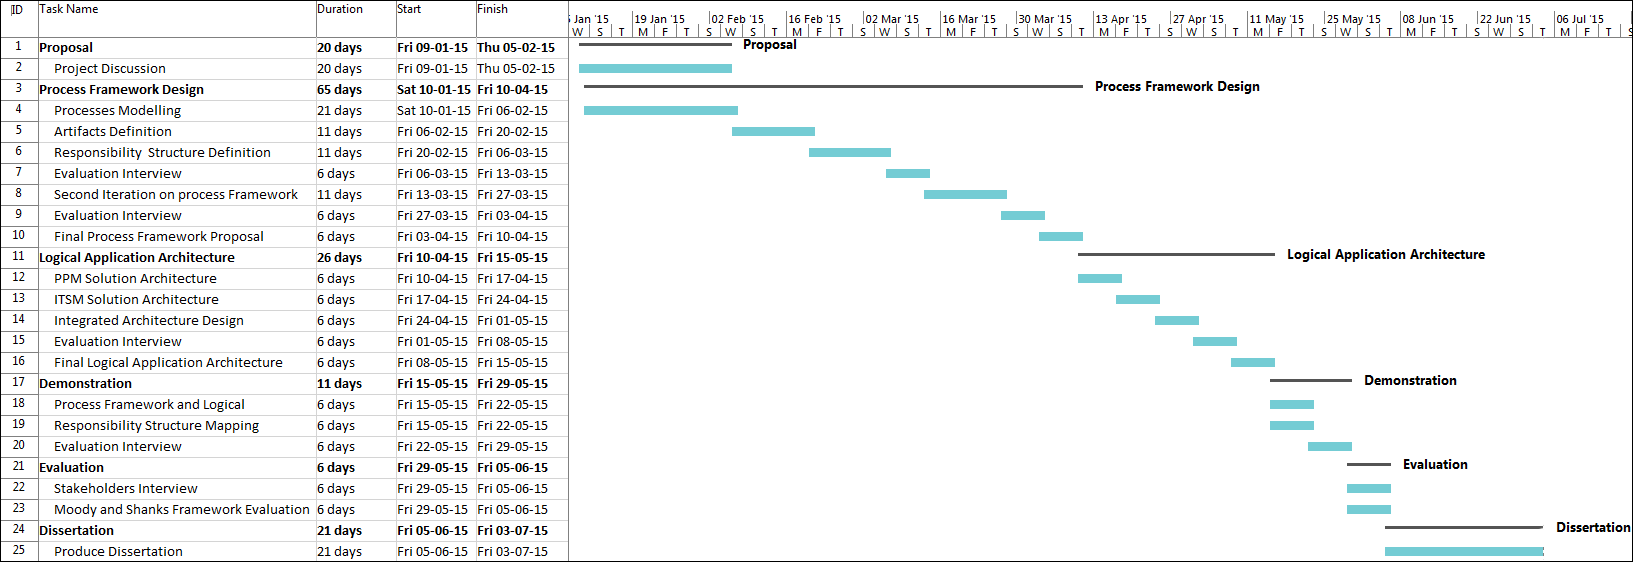
\includegraphics[height=0.55\textheight]{img/GanttChart.png}
\caption{Gantt Chart for the project.}
\end{figure}

\end{landscape}

\newpage



\begin{table}[h!]
\centering
\resizebox{\textwidth}{!}{%
\begin{tabular}{|l|l|}
\hline
\multicolumn{1}{|c|}{\textbf{Task ID}} & \multicolumn{1}{c|}{\textbf{Objectives}} \\ \hline
\rowcolor[HTML]{68CBD0} 
\textbf{1} & \textbf{Proposal} \\ \hline
2 & Prepare project presentation and discussion. \\ \hline
\rowcolor[HTML]{68CBD0} 
\textbf{3} & \textbf{Process Framework Design} \\ \hline
4 & \begin{tabular}[c]{@{}l@{}}Selection of high level processes to include in framework; \\ Definition of activities for each process; \\ Definition of objectives, inputs and outputs of each activity;\end{tabular} \\ \hline
5 & \begin{tabular}[c]{@{}l@{}}Definition of artifacts related to inputs and outputs of each activity; \\ Artifacts design and production;\end{tabular} \\ \hline
6 & \begin{tabular}[c]{@{}l@{}}Definition of a responsibility structure to support the processes;\\ Responsibility assignment;\end{tabular} \\ \hline
7 & \begin{tabular}[c]{@{}l@{}}Interview with the main stakeholder; \\ Necessary changes definition; \\ Evaluation Report;\end{tabular} \\ \hline
8 & \begin{tabular}[c]{@{}l@{}}Iteration on Processes modelling, Artifact definition and \\ responsibility structure definition tasks;\end{tabular} \\ \hline
9 & \begin{tabular}[c]{@{}l@{}}Interview with the main stakeholder; \\ Necessary changes definition; \\ Evaluation Report;\end{tabular} \\ \hline
10 & \begin{tabular}[c]{@{}l@{}}Iteration on Processes modelling, Artifact definition and responsibility\\ structure definition tasks; \\ Final proposal for the Process Framework;\end{tabular} \\ \hline
\rowcolor[HTML]{68CBD0} 
\textbf{11} & \textbf{Logical Application Architecture} \\ \hline
12 & \begin{tabular}[c]{@{}l@{}}Definition of PPM solution's features to include into the architecture; \\ Definition of input activities from process framework to PPM solution; \\ Definition of outputs from PPM Solution;\end{tabular} \\ \hline
13 & \begin{tabular}[c]{@{}l@{}}Definition of ITSM solution's features to include into the architecture; \\ Definition of,input activities from process framework to ITSM solution; \\ Definition of outputs from ITSM Solution;\end{tabular} \\ \hline
14 & \begin{tabular}[c]{@{}l@{}}Definition of ITSM and PPM solution's inputs from the processes framework; \\ Integration with application architectures already present in the organization; \\ Definition of application architecture outputs; \\ Definition of necessary infrastructure;\end{tabular} \\ \hline
15 & \begin{tabular}[c]{@{}l@{}}Interview with the main stakeholder; \\ Necessary changes definition; \\ Evaluation Report;\end{tabular} \\ \hline
16 & \begin{tabular}[c]{@{}l@{}}Iteration on ITSM and PPM solutions' architecture;\\ Final proposal for the Logical Application architecture;\end{tabular} \\ \hline
\rowcolor[HTML]{68CBD0} 
\textbf{17} & \textbf{Demonstration} \\ \hline
18 & \begin{tabular}[c]{@{}l@{}}Process framework and Logical Application Architecture presentation to stakeholders;\\ Process framework application proposal to the organization;\\ Logical application architecture integration on organization proposal;\end{tabular} \\ \hline
19 & Mapping between responsibility structure defined and demonstration's organization structure; \\ \hline
20 & \begin{tabular}[c]{@{}l@{}}Interview with the main stakeholder; \\ Evaluation Report;\end{tabular} \\ \hline
\rowcolor[HTML]{68CBD0} 
\textbf{21} & \textbf{Evaluation} \\ \hline
22 & \begin{tabular}[c]{@{}l@{}}Interview with the main stakeholder; \\ Evaluation Report;\end{tabular} \\ \hline
23 & \begin{tabular}[c]{@{}l@{}}Evaluation using Moody and Shanks Framework; \\ Results analysis and reporting;\end{tabular} \\ \hline
\rowcolor[HTML]{68CBD0} 
24 & \textbf{Dissertation} \\ \hline
25 & \begin{tabular}[c]{@{}l@{}}Write dissertation;\\ Dissertation presentation;\end{tabular} \\ \hline
\end{tabular}
}
\vspace{2mm}
\caption{Tasks and objectives for the project.}
\label{my-label}
\end{table}

\newpage

\subsection{Appendix B - COBIT 5 Processes by domain} 

The next figure presents the management and governance processes from COBIT 5 process framework, presented by domain.

\begin{figure}[h!]
\centering
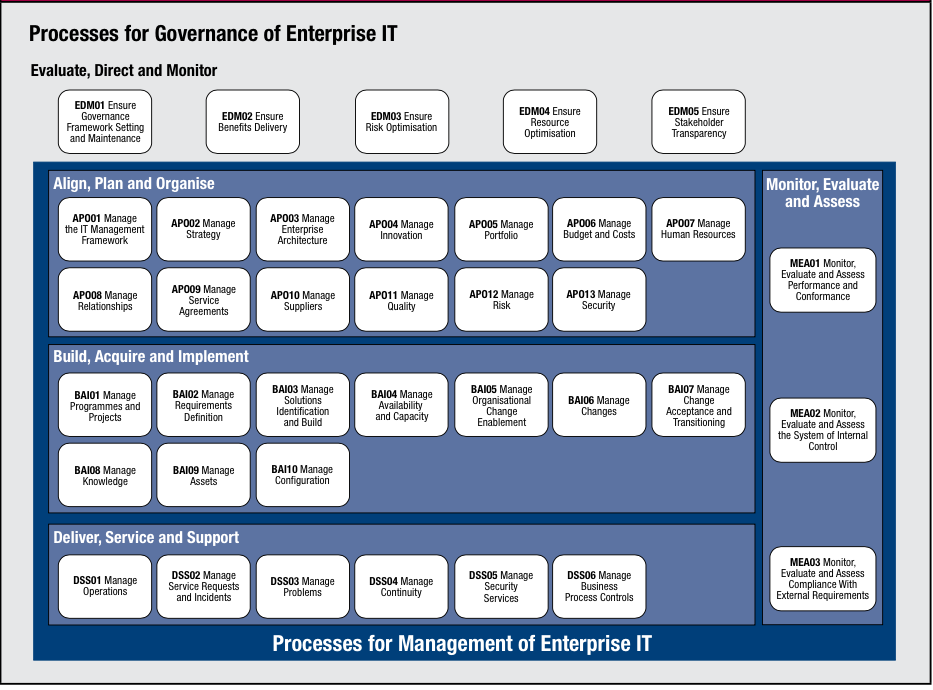
\includegraphics[width=\textwidth]{img/COBIT5ProcessFramework.png}
\caption{COBIT 5 Processes. Extracted from \cite{2012cobit}.}
\end{figure}

\newpage

\subsection{Appendix C - ISO 19011 Audit Programme Management process} 

The next figure presents the process flow purposed by ISO 19011 International standard for Audit programmes management.

\begin{figure}[h!]
\centering
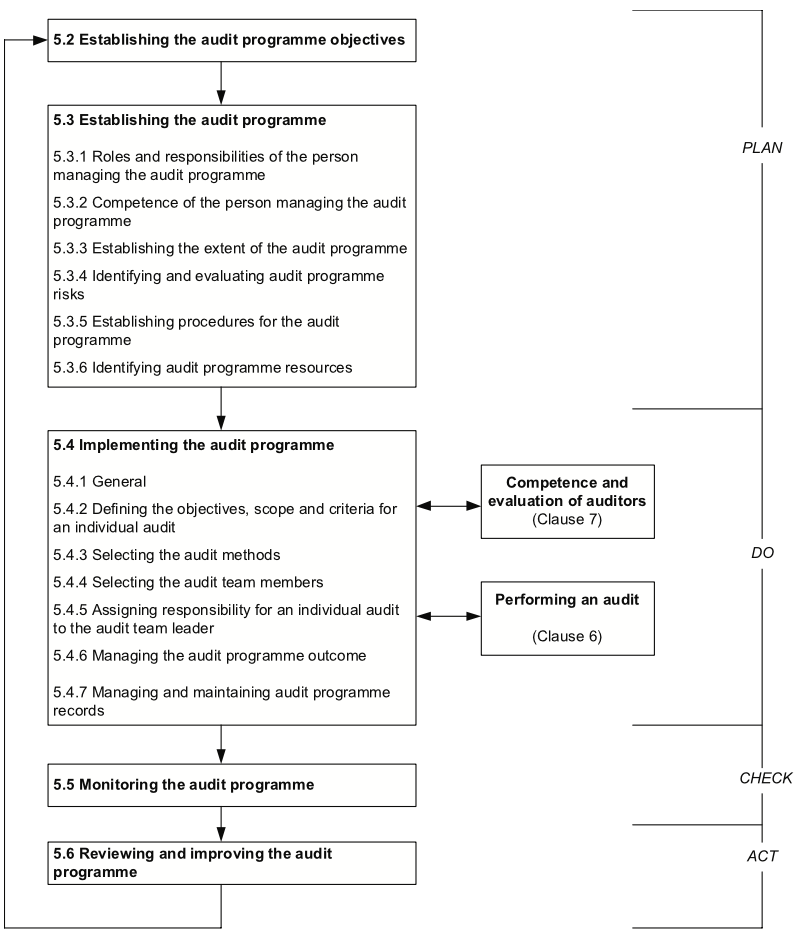
\includegraphics[width=0.9\textwidth]{img/ISO19011AuditProcess.png}
\caption{ISO 19011 Audit Programme Management process. Extracted from \cite{ISO19011}.}
\end{figure}





\newpage


% 
% Bibliography
% 
\bibliographystyle{plain} 

% replace example.bib with your .bib
\bibliography{refs.bib} 

\end{document}